\chapter{Related Works}

This chapter presents, in the first section, an overview of the different datasets available online for anomaly detection tasks. Next, different autoencoder-based architectures found in literature for anomaly detection are presented.

\section{Available datasets}
One of the main reasons for the success of ML or DL algorithms is the availability of more and more public standard datasets, regarded as common benchmarks and that allow a fair comparison between different proposals present in literature. In PdM and in anomaly detection tasks, this is not totally true, because often machinery data are confidential (so not publicly available) and sometimes studies are conducted by companies internal divisions. In response to the need of public dataset arranged for anomaly detection tasks, in the last years some datasets have been built and then made available online (Table \ref{datasets-table}).\\

% Please add the following required packages to your document preamble:
% \usepackage{booktabs}
\begin{table}[ht]
\small
\centering
\begin{tabularx}{\textwidth}{cl}
\hline
Dataset Name & Summary \\ \hline
CWRU & \begin{tabular}[c]{@{}l@{}}Ball bearing test data for normal and faulty bearings. \\ Motor bearings were seeded with faults using electro-discharge\\ machining (EDM) and vibration data was collected using \\ accelerometers, which were attached to the housing \\ with magnetic bases.\end{tabular} \\ \hline
MFPT & \begin{tabular}[c]{@{}l@{}}Provides time-series data from nominal, outer race fault at \\ various loads, inner race fault at various loads and three\\ real-world faults of bearings\end{tabular} \\ \hline
NAB & \begin{tabular}[c]{@{}l@{}}Contains cross-domain data collections, like \\ the average CPU usage in AWS cluster or the internal \\ temperature data of an industrial machine.\end{tabular} \\ \hline
Yahoo S5 & \begin{tabular}[c]{@{}l@{}}Consists of four data classes, each of which contains either a\\  set of synthetic or real web traffic metrics tagged with anomalies\end{tabular} \\ \hline
DCASE2020 & \begin{tabular}[c]{@{}l@{}}The dataset consists in sounds collected \\ from different industrial machines. It is composed by MIMII \\ Dataset and ToyADMOS.\end{tabular} \\ \hline
\end{tabularx}
\caption{Anomaly detection online available datasets.}
\label{datasets-table}
\end{table}
To clarify, these datasets contain some anomalous observations, often generated manually by operators, but, as mentioned in the first chapter, they not represents all the possible anomalous states. Anomalous observations are mainly used to build test set and consequently evaluate the performance of the models, trained in unsupervised way. 

\section{Anomaly detection with autoencoders}
In this section, some autoencoder-based architectures found in literature are presented.
Antonio L. Alfeo et al. \cite{12UsingAEinManufacturing} show an autoencoder-based approach using power consumption of industrial laundry assets and bearing vibrations data. In the first case, time-series are realistically created using official information provided by assets manufacturers (e.g. nominal energy consumption) and by researchers' industrial partner. In the second case, time-series are extracted from MFPT dataset presented in Table \ref{datasets-table}. After the creation of these ad-hoc datasets, the proposed approach employs an autoencoder to score the anomaly degree of each input instance, presented as rescaled time-series features. The reconstruction errors, calculated downstream of the decoder, are further processed by a discriminator, which rescales them between 0 and 1 by using a sigmoidal function (Figure \ref{autoencoder_plus_discriminator}).
\begin{figure}[ht]
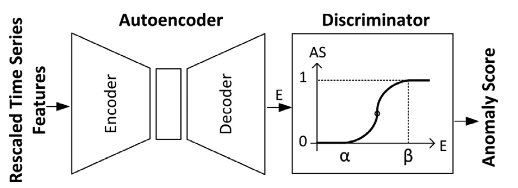
\includegraphics[scale=0.5]{TESI DI FIORE/img/Autoencoderplusdiscriminator.png}
\centering
\caption{Anomaly detector architecture proposed by \cite{12UsingAEinManufacturing}.}
\label{autoencoder_plus_discriminator}
\end{figure}
For both the dataset, the inputs of the architecture are samples characterized by statistical features extracted from time-series available in the dataset which capture their trends over time (like 90th, 75th, 50th and 25th percentile of the time series or the mean absolute deviation).\\
Ruei-Jie Hsieh et al \cite{9UnsupervisedOnlineAnomalyDetectionMultivariate} developed an unsupervised deep Recurrent Neural Network (RNN) detection model based on the Long Short Term Memory (LSTM) autoencoder. The recurrent layers of the autoencoder capture temporal dependencies in multivariate sensor data provided by a manufacturing company. The mentioned company has a production line in which there are three chambers (A,B,C) disposed in series and the product moves from a chamber to another. Each chamber has 4 sensors (W,X,Y,Z) for the detection of the products passage. When sensors outputs signal 1, it indicates the product is already in a chamber, otherwise it outputs 0. Obviously, the anomalies in data are not detectable in the single values generate by sensors, but only in the time sequence of them. This is the reason why the authors have chosen LSTM cells to build encoder and decoder layers. The detection of an anomalous behaviour in a chamber prevents that the products pass in the whole line when there is something wrong in the production process (early detection). Autoencoder models are trained to reconstruct input sequences, timestamp by timestamp, using a sliding-window method (sequence-to-sequence autoencoder), already analyzed in the first chapter. The input vector in each timestamp is composed by the readings of the four sensors in a chamber. Using a threshold $\epsilon$, defined through the reconstruction error of training data, each timestamp of each sequence is labeled as normal or anomalous on the basis of its reconstruction error. In conclusion, because each timestamp is labeled as many time as the sliding window length, a majority voting mechanism is applied to make the final decisions and eventually an alert is generated (Figure \ref{seq2seq-architecture}).\\
\begin{figure}[ht]
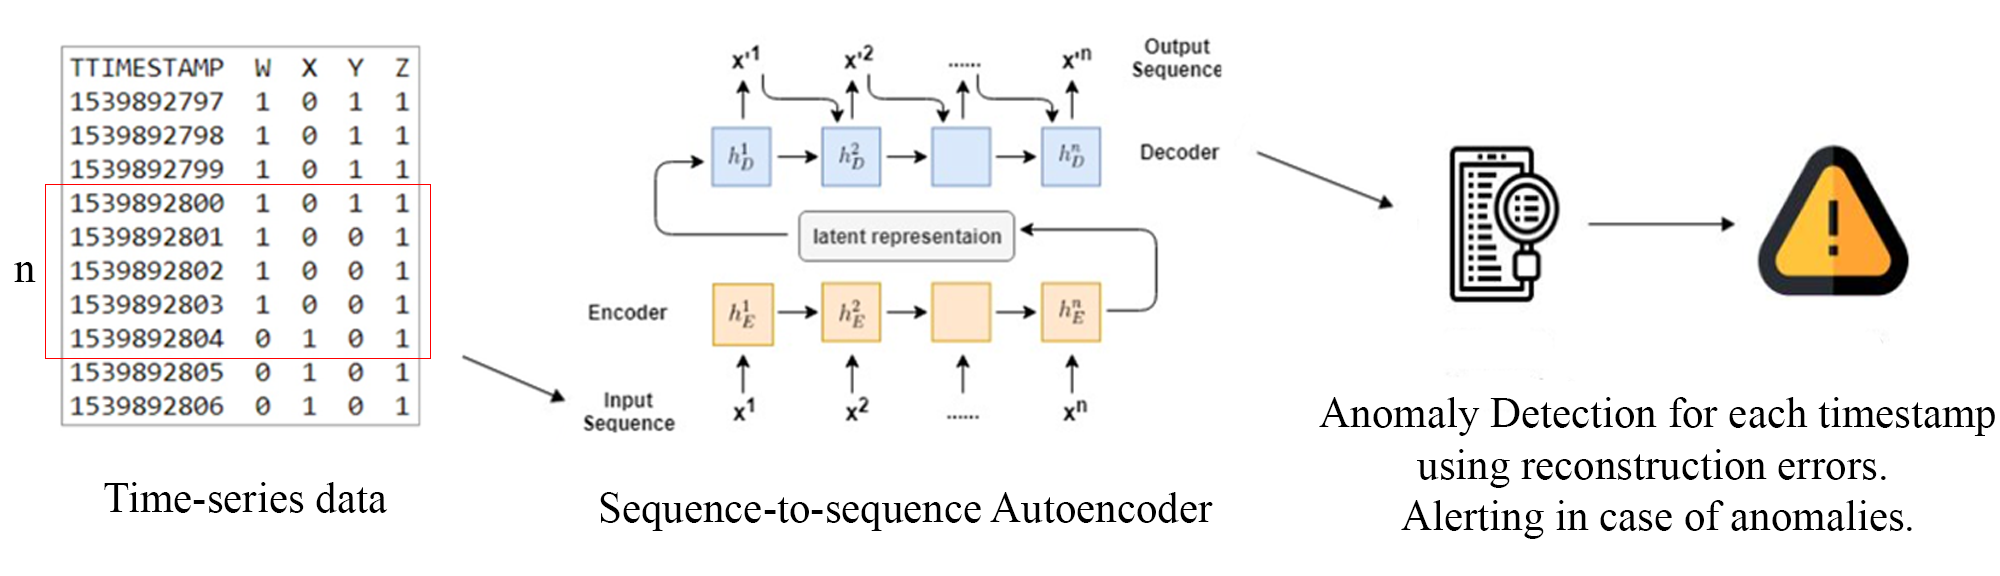
\includegraphics[scale=0.9]{TESI DI FIORE/img/sequence-to-sequecen-ae-anomalydetection.png}
\centering
\caption{Architecture pipeline proposed by \cite{9UnsupervisedOnlineAnomalyDetectionMultivariate}.}
\label{seq2seq-architecture}
\end{figure}\\
Another strategy to resolve the anomaly detection task is to combine deep learning and ensemble learning. Shao Haidong et al. \cite{14NovelMethodEnsembleDeepAutoencoder} propose a novel method called ensemble deep autoencoders (EDAEs) for the intelligent fault diagnosis of bearings, using CWRU dataset. The ensemble of multiple deep autoencoders is a good choice to overcome the low generalization ability of individual deep autoencoders. Diversification is obtained by designing deep autoencoders with different kind of activation functions, considering that neural networks differing in activation functions usually show different characteristics and complementary learning behaviours. As for the combination strategy, the authors define a new one. Firstly, for each deep autoencoder the classification accuracy is calculated and then compared to a pre-defined threshold. Next, only autoencoders with accuracy greater than the threshold are kept, then different weights are calculated and assigned to each model using its accuracy. Finally, the achitecture reports the combined diagnosis result of each sample based on the weight scores. In order to maintain the stability of the combined diagnosis results, repeated trials are carried out. The results, in terms of precision, recall and F-Measure, demonstrate the validity of this architecture.\\
Chen et al. \cite{21RobotAnomalyDetection} introduce an unsupervised anomaly detection system for industrial robots, based on a sliding-window convolutional variational \footnote{Differently from classical autoencoders, in VAE, the latent variable z is constrained to be distributed according to a prior distribution $p_\theta (z)$, usually multivariate unit Gaussian $\mathcal{N}(0,I)$, forcing the model to learn the distribution of input data.}
autoencoder (SWCVAE), which realizes real-time anomaly detection by coping with multivariate time series data. Their architecture can be also used for online anomaly detection and it can be trained in unsupervised manner. To validate the approach, KUKA KR6R 900SIXX is chosen by the authors, which is an industrial robot with six revolute joints that repeatedly performs a pick-and-place task using vision guidance system. The authors record the joint angles and joint currents of the six joints of the robot at 33.3 Hz from the robot controller, so without using external sensor devices but only the data provided by the robot itself. For testing purpose, in order to simulate faults, collisions have been induced by manually hitting the robot.

\section{Anomalous Sound Detection (ASD)}
The existing anomaly detection systems used in the industrial domain depend, obviously, on the properties of sensors used to monitor an industrial machine. Among those systems, most common are visual anomaly detection systems, which have some drawbacks such as illumination, occlusion by objects, being out of the field of view and so forth, which strongly affect the performance of the system, especially in terms of computation power needed to achieve high real time performances. ASD systems, however, are not affected by the problems just described. In fact, the use of acoustic data features also offers an advantage in terms of simplicity in data retrieval. On the other hand, compared to images, audio clips need some pre-processing steps to be converted in different formats compatible with neural network training process, like signals representing air pressure values or spectrograms, often in the Mel scale\footnote{In Mel-Scale the entire frequency spectrum is separated into $x$ evenly spaced frequencies (bins), where 'evenly spaced' means that the distance on the frequency dimension approximates the human auditory system’s response more closely than the linearly-spaced frequency bands used normally in spectrograms}.\\
In this context, the authors of \cite{13RealTimeDetectionUsingSequentialAutoencoder} compare the performances of convolutional LSTM autoencoder (Conv-LSTMAE)  and sequential convolutional autoencoder (CAE) using sounds retrieved from Youtube videos recorded during industrial manufacturing processes. Because it is hard to capture abnormal patterns due to their rarity in real life and because the creation of anomaly events and recording respective sounds is expensive, the authors generate artificially anomalous samples for testing adding anomaly events like explosion, fire or glass breaking to downloaded clips. Although the proposed two autoencoders are different in terms of layers, the pipeline of the system is fixed: there are sequences of five 128x128 spectrograms (extracted from audio dataset) that are the inputs of a sequential autoencoder, which generate output sequences that must be as much similar as possible to the input ones. Also this time, the decision about the generation of an alert due to the possible presence of anomalies, is made on the comparison between the reconstruction error of each spectrogram and a pre-defined threshold (Figure \ref{seq2seq-architecture-realtime}).

\begin{figure}[ht]
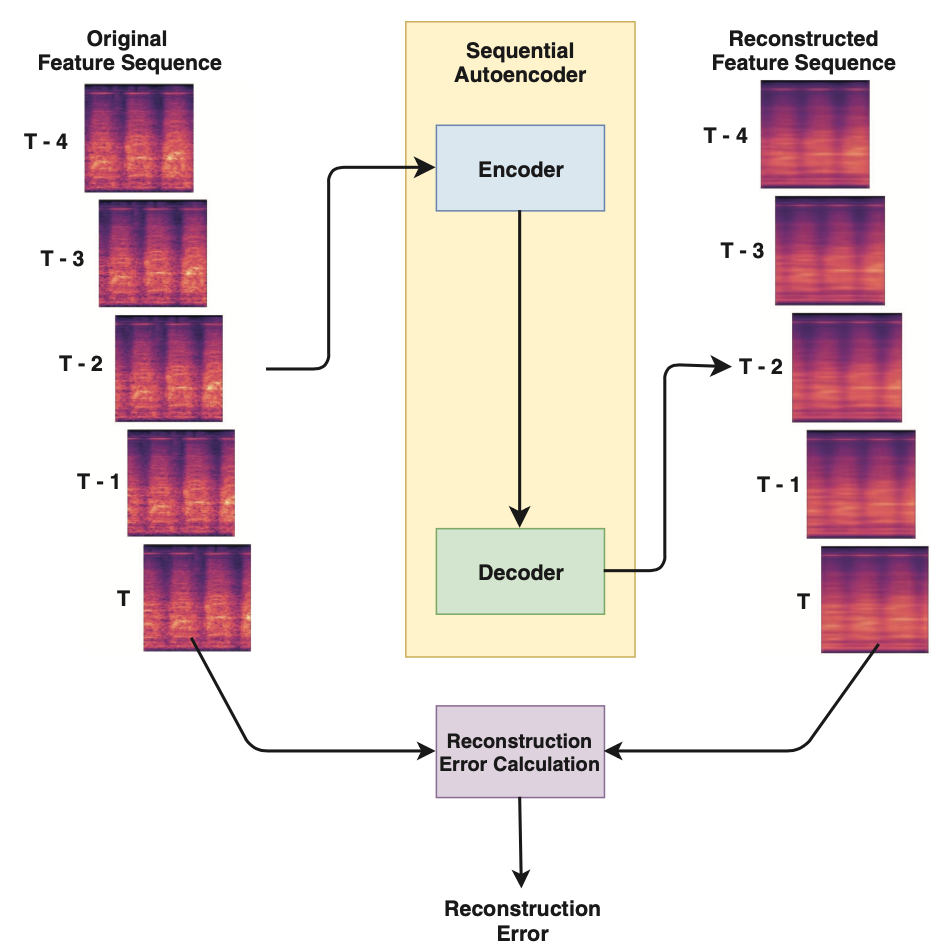
\includegraphics[scale=0.4]{TESI DI FIORE/img/SeqToSeqAutoencoderRealTimeDetection.png}
\centering
\caption{The reconstruction and reconstruction error calculation stages \cite{13RealTimeDetectionUsingSequentialAutoencoder}}
\label{seq2seq-architecture-realtime}
\end{figure}

Another paper in which the reconstruction error of a pre-trained autoencoder is used for anomaly detection using sound data, is the one proposed by Dong Yul Oh et al. \cite{22SMDMachineResidualError}. They propose a convolutional autoencoder which receives in input frames of size 1024x32, obtained after a segmentation of mel spectrograms extracted from an audio dataset. The particularity of this work is in how the authors validate their approach. They use a real Surface-Mount Device (SMD) assembly machine, which performs a dozen operations in a second. Since the microphones are disposed really close to the machine, additional processing for the ambient noise is not required. The entire machine production in their experimental data consists of two lines (B and C), which differ in terms of which semiconductors are being assembled. C-Line is used as a normal category and all others are assumed to be abnormal (one vs. all). They manually defined three abnormal categories: changing assembly part (from C-Line to B-line), adding noise artificially (to represent broken internal components) and removing grease in the same production C-line. The details of the convolutional architecture are shown in the Figure \ref{22ConvAEArchitecture}.

\begin{figure}[ht]
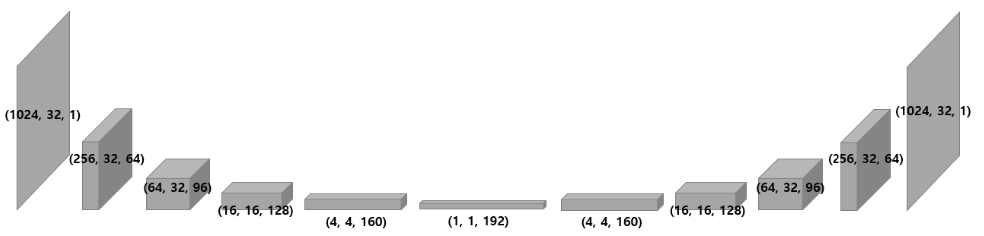
\includegraphics[scale=0.8]{TESI DI FIORE/img/22ArchitectureConvAE.png}
\centering
\caption{Overall structure of convolutional autoencoder proposed by the authors of \cite{22SMDMachineResidualError}.}
\label{22ConvAEArchitecture}
\end{figure}

The case study of the SMD machine was brought forward in \cite{23SMDFared}, in which a model, called FARED is presented. FARED stands for Fast Adaptive RNN Encoder–Decoder and it is a new recurrent approach used for anomaly detection. Here, autoencoder is built using LSTM for each RNN cell.

\begin{figure}[ht]
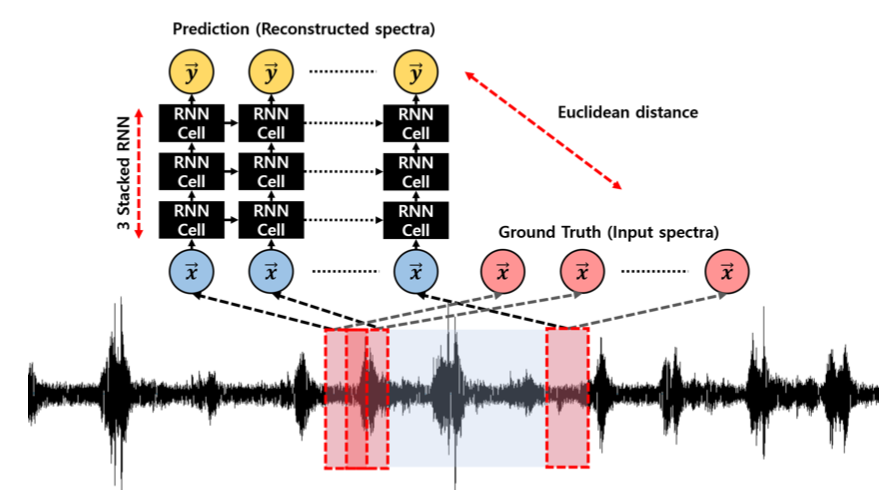
\includegraphics[scale=0.8]{TESI DI FIORE/img/23FARED.png}
\centering
\caption{Structure of Fast Adaptive Recurrent Neural Network (RNN) Encoder–Decoder (FARED) \cite{23SMDFared}.}
\label{23FARED}
\end{figure}

The Figure \ref{23FARED} shows that the input is constructed by sequential spectrum (red box) and that each spectrum has 50\% of overlapping in the time domain. The output is a sequential reconstructed spectrum from input sequences. The Euclidean distance between prediction and ground truth is used for training and anomaly detection. The main objective pursued with the introduction of this recurrent architecture is the training time reduction, since this type of machine is used in different small productions, dedicated to different target products. In fact, the production features often changes and models must be trained easily and as soon as possible. Both the autoencoder tested on SMD machine uses the threshold mechanism to eventually generate alerts.\\
Very interesting is the study conducted by Maarten Meire and Peter Karsmakers \cite{24ComparisonDeepAutoencodersRealTime}. They propose two approaches: one based on One-Class Support Vector Machine (OC-SVM) and one based on autoencoders trained in unsupervised way. The novelty brought in this paper does not reside so much in how the models are trained or built, but in their efficiency, in terms of accuracy but also in computational power. In fact, the main focus is often to increase the difference between the reconstruction errors of normal and anomalous data, without considering training performances and speed, but if it is necessary to bring the trained system to the edge (on sensors themselves or close to them) computational power is a factor to be monitored carefully. This study is conducted comparing different implementations of convolutional neural network autoencoders and OC-SVM approach, using acoustic data collected from healthy and faulty bearings generated with Siemens Industry Software, pre-processed to generate spectrograms in mel scale, similarly as seen in previously analyzed works. This comparison, in terms of models accuracy, training times and number of algorithms parameters, is done twice, when the microphone is close to the faulty bearing and when it is far from it. Conclusions drawn by the authors highlight that the best compromise between accuracy and performance on hardware for real-time detection is represented by the 2D-CNN autoencoder.\\
When an ASD system overlooks an anomaly, an update of the system is necessary to never overlook the observed type of anomalies twice. There are two ways to face this problem: re-training the whole system using all training data, or cascading a new specific detector for the overlooked anomaly. The first approach is the most effective solution but an huge computational cost and an amount of anomalous training data are required to re-train the system. In \cite{25SNIPER} the second one is tried, with a few-shot learning method for ADS. The authors propose and architecture called SNIPER (“few-Shot learNIng with ensured true-PositivE-Rate), whose goal is to maximize the true positive rate (TPR) on the observed anomaly, but the problem is the absence of an huge amount of data related to it (Figure \ref{SNIPER}). The solution found by the authors is the following: they combine the anomaly score produced by an autoencoder trained in unsupervised manner and a new ad-hoc similarity score, produced by a specific anomaly detector $\mathcal{S}$ on the basis of a comparison between input samples and memorized anomalous sounds (overlooked in the past). The authors build $\mathcal{S}$ using an approach based on VAE, to overcome the problem of the absence of sufficient overlooked anomalous data.
\begin{figure}[ht]
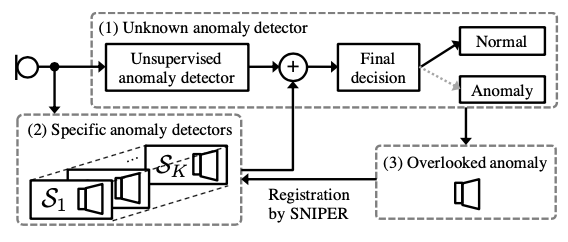
\includegraphics[scale=1]{TESI DI FIORE/img/SNIPER.png}
\centering
\caption{High level view of SNIPER. Overlooked anomalous sound is registered to specific anomaly detector with proposed method. \cite{25SNIPER}}
\label{SNIPER}
\end{figure}
\subsection{DCASE Challenge: an ASD task}
Detection and Classification of Acoustic Scenes and Events, is a community that organizes challenges every year and usually their task 2 regards predictive maintenance with audio clips as dataset. The dataset presented in the Table \ref{datasets-table} is provided by DCASE 2020 Challenge, whose title is "\textit{unsupervised detection of anomalous sounds for machine condition monitoring}". Because of only normal working machines sound samples are provided as training data (in form of clips, lasting 10 or 11 seconds), the task is already arranged to be resolved in unsupervised way, and, again, autoencoder is one of the best techniques. In details, the dataset that can be downloaded is composed by ToyADMOS Dataset and MIMII Dataset \cite{DCASE} and refers to different sounds recorded with microphones disposed around different machine types: a toy-car, a toy-conveyor, a valve, a pump, a fan and a slide rail. To make the challenge more interesting, different machines for each type are considered, identified by an ID string (for example different kinds of pump). A baseline system implementation for comparison purpose was made available by the authors of the challenge. It consists of a dense autoencoder with three layers, in both the encoder and decoder components, with 128 units, and a latent space with 8 units, all with the ReLU activation function. Following, a summary of most interesting approaches for the improvement of the baseline system is shown, while, in the next chapters, the dataset is explored more in details to support a better explaination of the experimental part of this text.\\
% LITERATURE
Pilastri et al. \cite{15DeepDenseConvAE} propose two deep learning models, based on a dense and convolutional architectures fed with spectrograms. For the dense one, the encoder and decoder networsks consist of four fully-connected layers, followed by Batch Normalization and ReLU as the activation function. For the convolutional one, the encoder and decoder networks are composed by convolutional layers with Batch Normalization and the ReLU activation function after each convolution. In both architectures the goal is to minimize the reconstruction error between inputs and outputs. Regarding features extraction, for the dense autoencoder, audio samples are buffered in fixed-length 1 second intervals with a 50\% overlap and, after the extraction of spectrograms 128x640 dimensional input matrix are obtained. In the convolutional autoencoder system, the spectrograms obtained from samples are segmented to form 128x32 frames, ready for training. As for previous described architectures, the classification of audio clips, is made comparing the reconstruction error (in terms of MSE) and a pre-defined threshold. Results show that for two machine types (slider and valve), the best results were achieved by the convolutional autoencoder, while the dense autoencoder provided the best results for the others.\\
Again, also in anomalous sound detection task, some LSTM-based autoencoders architecture can be found in literature. For example, in the technical report provided by Jalali et al. \cite{16LSTMDeepAutoencodersForASDtask}, the architecture encodes the information using LSTM layers with \textit{n} units and then their outputs are passed into a bottleneck layer, which is also a LSTM layer with smaller size together with a repeat vector layer. A repeat vector layer repeats its input vector multiple times (the number of time steps chosen for the sequences). Next, a stack of sequential LSTM layers reconstruct the original input.\\
Another interesting approach is the one proposed by Tomoki Hayashi et al. \cite{17ConformerBasedIDAWAREAutoencoder}. Their paper presents a Transformer-based and Conformer-based autoencoder for ASD, performing sequence-to-sequence processing. With respect to the standard autoencoder, this kind of architectures can extract sequence-level information from whole audio inputs, using a methodology called self-attention mechanism, with whom Trasformer and Conformer neural networks are built. In fact, a critical disadvantage of classic sequence-to-sequence autoencoder is the inability of the system to retain longer sequences. The attention mechanism was created to resolve this problem of long dependencies, as it is an interface connecting the encoder and decoder providing to the decoder the information from every encoder hidden state. With this framework, the model is able to selectively focus on valuable parts of the input sequence and hence, learn the association between them.\\
As can be noted, all the approaches proposed above differ from the way autoencoders are built. In fact, the main idea is always to train autoencoders to reconstruct as well as possible the normal audio samples provided in input and then to detect anomalies when there is some inputs that are badly reconstructed by the architecture. In literature, however, there are also some proposals that are regardless of how the autoencoders are build. For example, the authors of \cite{18IDConditionedAutoEncoder}\cite{19DescriptionDiscussionDCASE2020} and also the same researchers of the last presented approach, introduce the concepts of ID conditioning and ID regression. The main idea of both is to use the information related to the particular device identifier from which the input sound clips are retrieved to influence the autoencoder behaviour. 